\newpage
\section{Контрольная работа 1}


% \subsection[что идет в оглавление]{\hyperref[на что ссылка]{текст ссылки}}
\subsection[2017-2018]{\hyperref[sec:sol_kr_01_2017_2018]{2017-2018}}
\label{sec:kr_01_2017_2018} % \label{ссылка сюда}

% * — не идёт в оглавление
\subsubsection*{Минимум}

\begin{enumerate}
\item Функция распределения случайной величины: определения и свойства.
\item Экспоненциальное распределение: определение, математическое ожидание и дисперсия.
\item В операционном отделе банка работает 80\% опытных сотрудников и 20\% неопытных. Вероятность совершения ошибки при очередной банковской операции опытным сотрудником равна $0.01$, а неопытным — $0.1$. Известно, что при очередной банковской операции была допущена ошибка. Найдите вероятность того, что ошибку допустил неопытный сотрудник.
\item При работе некоторого устройства время от времени возникают сбои. Количество сбоев за сутки имеет распределение Пуассона. Среднее количество сбоев за сутки равно 3. Найдите вероятность того, что за двое суток не произойдет ни одного сбоя.

\end{enumerate}

\subsubsection*{Задачи}

\begin{enumerate}

\item Правильный кубик подбрасывают один раз. Событие $A$ — выпало чётное число, событие $B$ — выпало число кратное трём, событие $C$ — выпало число, большее трёх.

\begin{enumerate}
\item Сформулируйте определение независимости двух событий;
\item Определите, какие из пар событий $A$, $B$ и $C$ будут независимыми.
\end{enumerate}


\item Теоретический минимум (ТМ) состоит из 10 вопросов, задачный (ЗМ) — из 24 задач.
Каждый вариант контрольной содержит два вопроса из ТМ и две задачи из ЗМ.
Чтобы получить за контрольную работу оценку 4 и выше, необходимо и достаточно правильно ответить на каждый вопрос ТМ и задачу ЗМ доставшегося варианта. Студент Вася принципиально выучил только $k$ вопросов ТМ и две трети ЗМ.
\begin{enumerate}
\item Сколько всего можно составить вариантов, отличающихся хотя бы одним заданием в ТМ или ЗМ части? Порядок заданий внутри варианта не важен.
\item Найдите вероятность того, что Вася правильно решит задачи ЗМ;
\item Дополнительно известно, что Васина вероятность правильно ответить на вопросы ТМ, составляет $1/15$. Сколько вопросов ТМ выучил Вася?
\end{enumerate}

\item Производитель молочных продуктов выпустил новый низкокалорийный йогурт Fit и утверждает, что он вкуснее его более калорийного аналога Fat.
Четырем независимым экспертам предлагают выбрать наиболее вкусный йогурт из трёх, предлагая им в одинаковых стаканчиках в случайном порядке два Fat и один Fit.
Предположим, что йогурты одинаково привлекательны.
Величина $\xi$ — число экспертов, отдавших предпочтение Fit.
\begin{enumerate}
\item Какова вероятность, что большинство экспертов выберут Fit?
\item Постройте функцию распределения величины $\xi$;
\item Каково наиболее вероятное число экспертов, отдавших предпочтение йогорту Fit?
\item Вычислите математическое ожидание и дисперсию $\xi$.
\end{enumerate}

\item Дядя Фёдор каждую субботу закупает в магазине продукты по списку, составленному котом Матроскином. Список не изменяется, и в него всегда входит 1 кг сметаны, цена которого является равномерно распределённой величиной $\alpha$, принимающей значения от 250 до 1000 рублей. Стоимость остальных продуктов из списка в тысячах рублей является случайной величиной $\xi$ с функцией распределения

\[
F(x)=\begin{cases}
1-\exp(-x^2 ), \text{ если } x \geq 0 \\
0, \text{ иначе.}\\
\end{cases}
\]

\begin{enumerate}
\item Какую сумму должен выделить кот Матроскин дяде Фёдору, чтобы её достоверно хватало на покупку сметаны?
\item Какую сумму должен выделить кот Матроскин дяде Фёдору, чтобы Дядя Фёдор с вероятностью 0.9 мог оплатить продукты без сметаны?
\item Найдите математическое ожидание стоимости продуктов без сметаны;
\item Найдите математическое ожидание стоимости всего списка.
\item Какова вероятность того, что общие расходы будут в точности равны их математическому ожиданию?
\end{enumerate}

Подсказка: $\int_0^{\infty} \exp(-x^2) \, dx = \sqrt{\pi} / 2$.

\item Эксперт с помощью детектора лжи пытается определить, говорит ли подозреваемый правду. Если подозреваемый говорит правду, то эксперт ошибочно выявляет ложь с вероятностью 0.1. Если подозреваемый обманывает, то эксперт выявляет ложь с вероятностью 0.95.

В деле об одиночном нападении подозревают десять человек, один из которых виновен и будет лгать, остальные невиновны и говорят правду.

\begin{enumerate}
\item Какова вероятность того, что детектор покажет, что конкретный подозреваемый лжёт?
\item Какова вероятность того, что подозреваемый невиновен, если детектор показал, что он лжёт?
\item Какова вероятность того, что эксперт точно выявит преступника?
\item Какова вероятность того, что эксперт ошибочно выявит  преступника, то есть покажет, что лжёт невиновный, а все остальные говорят правду?
\end{enumerate}
\end{enumerate}


\newpage
\subsection[2016-2017]{\hyperref[sec:sol_kr_01_2016_2017]{2016-2017}}
\label{sec:kr_01_2016_2017}

\begin{enumerate}
\item Из семей, имеющих двоих разновозрастных детей, случайным образом выбирается одна семья.
Известно, что в семье есть девочка (событие $A$).

\begin{enumerate}
\item	Какова вероятность того, что в семье есть мальчик (событие $B$)?
\item	Сформулируйте определение независимости событий и проверьте,
являются ли события $A$ и $B$ независимыми?
\end{enumerate}

\item Система состоит из $N$ независимых узлов.
При выходе из строя хотя бы одного узла, система дает сбой.
Вероятность выхода из строя любого из узлов равна $0.000001$.
Вычислите максимально возможное число узлов системы,
при котором вероятность её сбоя не превышает $0.01$.

\item Исследование состояния здоровья населения в шахтерском регионе
«Велико-кротовск» за пятилетний период показало,
что из всех людей с диагностированным заболеванием легких, 22\% работало на шахтах.
Из тех, у кого не было диагностировано заболевание легких, только 14\% работало на шахтах.
Заболевание легких было диагностировано у 4\% населения региона.

\begin{enumerate}
\item	Какой процент людей среди тех, кто работал в шахте,
составляют люди с диагностированным заболеванием легких?
\item	Какой процент людей среди тех, кто НЕ работал в шахте,
составляют люди с диагностированным заболеванием легких?
\end{enumerate}

\item  Студент Петя выполняет тест (множественного выбора) проставлением ответов наугад.
В тесте 17 вопросов, в каждом из которых пять вариантов ответов и только один из них правильный.
Оценка по десятибалльной шкале формируется следующим образом:
\[
\text{Оценка} =
\begin{cases}
\text{ЧПО} - 7, & \text{если $\text{ЧПО}\in [8;\,17]$,} \\
1,              & \text{если $\text{ЧПО}\in [0;\,7]$}
\end{cases}
\]
где ЧПО означает число правильных ответов.

\begin{enumerate}
\item	Найдите наиболее вероятное число правильных ответов.
\item	Найдите математическое ожидание и дисперсию числа правильных ответов.
\item	Найдите вероятность того, что Петя получит «отлично»
(по десятибалльной шкале получит 8, 9 или 10 баллов).

Студент Вася также выполняет тест проставлением ответов наугад.

\item	Найдите вероятность того, что все ответы Пети и Васи совпадут.
\end{enumerate}

\item  Продавец высокотехнологичного оборудования контактирует с одним или двумя
потенциальными покупателями в день с вероятностями $1/3$ и $2/3$ соответственно.
Каждый контакт заканчивается «ничем» с вероятностью $0.9$ и покупкой оборудования
на сумму в 50\,000 у.\,е. с вероятностью $0.1$.
Пусть $\xi$ — случайная величина, означающая объем дневных продаж в у.\,е.

\begin{enumerate}
\item	Вычислите  $\P(\xi = 0)$.
\item	Сформулируйте определение функции распределения и постройте функцию распределения
случайной величины $\xi$.
\item	Вычислите математическое ожидание и дисперсию случайной величины $\xi$.
\end{enumerate}

\item Интервал движения поездов метро фиксирован и равен $b$ минут,
т.е. каждый следующий поезд появляется после предыдущего ровно через $b$ минут.
Пассажир приходит на станцию в случайный момент времени.
Пусть случайная величина $\xi$, означающая время ожидания поезда,
имеет равномерное распределение на отрезке $[0; b]$.

\begin{enumerate}
\item Запишите плотность распределения случайной величины $\xi$.
\item	Найдите константу $b$, если известно, что в среднем пассажиру приходится
ждать поезда одну минуту, т.\,е. $\E(\xi) = 1$.
\item	Вычислите дисперсию случайной величины $\xi$.
\item	Найдите вероятность того, что пассажир будет ждать поезд менее одной минуты.
\item	Найдите квантиль порядка $0.25$ распределения случайной величины $\xi$.
\item	Найдите центральный момент порядка 2017 случайной величины $\xi$.
\item	Постройте функцию распределения случайной величины $\xi$.

Марья Ивановна из суеверия всегда пропускает два поезда и садится в третий.

\item	Найдите математическое ожидание и дисперсию времени,
затрачиваемого Марьей Ивановной на ожидание «своего» поезда.

Глафира Петровна не садится в поезд, если видит в нем подозрительного человека.
Подозрительные люди встречаются в каждом поезде с вероятностью $3/4$.

\item	Найдите вероятность того, что Глафире Петровне придется ждать не менее пяти минут,
чтобы уехать со станции.
\item	Найдите математическое ожидание времени ожидания «своего» поезда для Глафиры Петровны.
\end{enumerate}

\item (Бонусная задача)
На первом этаже десятиэтажного дома в лифт заходят 9 человек.
Найдите математическое ожидание числа остановок лифта, если люди выходят из лифта независимо друг от друга.
\end{enumerate}


\newpage
\subsection[2015-2016]{\hyperref[sec:sol_kr_01_2015_2016]{2015-2016}}
\label{sec:kr_01_2015_2016}

\begin{enumerate}
\item
Подбрасываются две симметричные монеты. Событие $А$ — на первой монете выпал
герб, событие $В$ — на второй монете выпал герб, событие $С$ — монеты выпали
разными сторонами.
\begin{enumerate}
    \item[$\alpha$)] Будут ли эти события попарно независимы?
    \item[$\beta$)]  Сформулируйте определение независимости в совокупности для трех событий. Являются ли события $A$, $B$, $C$ независимыми в совокупности?
\end{enumerate}

\item
Имеются два игральных кубика:
\begin{itemize}
    \item красный со смещенным центром тяжести, так что вероятность выпадения «6»
    равняется $1/3$, а оставшиеся грани имеют равные шансы на появление
    \item честный белый кубик
\end{itemize}

\begin{enumerate}
    \item[$\alpha$)] Петя случайным образом выбирает кубик и подбрасывает его.
    Найдите вероятность того, что выпадет «6».
    \item[$\beta$)]   Петя случайным образом выбирает кубик и подбрасывает его.
    Какова вероятность того, что Петя взял красный кубик, если известно, что выпала
    шестерка?
\end{enumerate}

\item
Все те же кубики. Петя играет с Васей в следующую игру: Петя выбирает кубик и
подбрасывает его. Вася подбрасывает оставшийся кубик. Выигрывает тот, у кого
выпало большее число. Если выпадает равное число очков, выигрывает тот, у кого
белый кубик.

Пусть случайная величина $\xi$ — число очков, выпавших на красном кубике,
случайная величина $\eta$ — число очков,
выпавших на белом кубике, а величина $\zeta$ — максимальное число очков.

\begin{enumerate}
    \item[$\alpha$)] Задайте в виде таблицы совместное распределение величин $\xi$ и $\eta$.
    Отметьте (* или кружочком) все те пары значений, когда выигрывает красный кубик.
    \item[$\beta$)] Какой кубик нужно выбрать Пете, чтобы его шансы выиграть были выше?
    \item[$\gamma$)] Сформулируйте определение функции распределения и постройте функцию
    распределения величины $\zeta$.
    \item[$\delta$)] Вычислите математическое ожидание величины $\zeta$.
\end{enumerate}

\item
Проводится исследование с целью определения процента мужчин, которые любят
петь в душе. Поскольку некоторые мужчины стесняются прямо отвечать на этот
вопрос, предлагается перед ответом на вопрос: «поете ли Вы, когда принимаете
душ?» подбросить правильный кубик, и выбрать ответ «ДА», если выпала
шестерка, ответ «НЕТ», если выпала единица, и честный ответ («ДА» или «НЕТ»),
если выпала любая другая цифра.

Предположим, что по результатам исследования
вероятность ответа «ДА» составляет $2/3$. Каков истинный процент «певцов»?

\item
Ваш полный тезка страдает дисграфией. При подписывании контрольной работы
по теории вероятностей в своих имени и фамилии в именительном падеже Ваш
тезка с вероятностью $0.1$ вместо нужной буквы пишет любую другую (независимо
от предыдущих ошибок).

\begin{enumerate}
    \item[$\alpha$)] Найдите вероятность того, что он напишет свою фамилию правильно.
    \item[$\beta$)] Найдите вероятность того, что он сделает ровно 2 ошибки в своем имени.
    \item[$\gamma)$] Вычислите наиболее вероятное число допущенных тезкой ошибок.
    \item[$\delta$)] Найдите вероятность того, что при подписывании работы Ваш тезка
    допустит хотя бы одну ошибку.
\end{enumerate}

\item
Время (в часах), за которое студенты выполняют экзаменационное задание
является случайной величиной с функцией плотности

\[
f(y) =
\begin{cases}
cy^2 + y , & \mbox{if } 0 \le y \le 1 \\
0, & \mbox{else}
\end{cases}
\]

\begin{enumerate}
    \item[$\alpha$)] Найдите константу $c$.
    \item[$\beta$)]  Найдите функцию распределения и постройте её.
    \item[$\gamma)$] Вычислите вероятность того, что случайно выбранный студент
    закончит работу менее чем за полчаса.
    \item[$\delta$)] Найдите медиану распределения.
    \item[$\epsilon$)] Определите вероятность того, что студент, которому требуется
    по меньшей мере 15 минут для выполнения задания, справится с ним более, чем за 30 минут.
\end{enumerate}

\item
Вам известно, что на большом листе бумаги $1.5$ м $\times$ $1$ м нарисован слон. Вам завязали
глаза и выдали кисточку хвоста для слона. Вам нужно прилепить эту кисточку к
листу (рисунок Вы не видели). Вы подходите к листу и произвольно приклеиваете
кисточку
\begin{enumerate}
    \item[$\alpha$)] Какова вероятность того, что кисточка окажется на слоне,
    если площадь рисунка составляет $1$ м$^2$?
    \item[$\beta$)] Запишите вид функции совместной плотности для координат кисточки.
    \item[$\gamma)$] Запишите вид частных функций плотности для каждой из координат кисточки.
    \item[$\delta$)] Являются ли координаты кисточки независимыми случайными величинами?
    \item[$\epsilon$)] Запишите вид функции плотности суммы координат кисточки.
\end{enumerate}
\textit{Подсказка: слон не должен заслонить равномерного распределения.}

\begin{center}
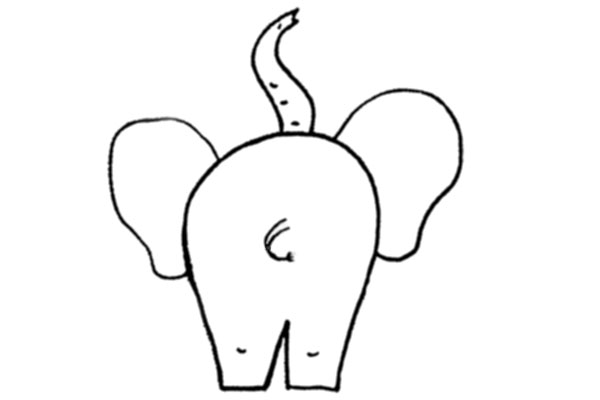
\includegraphics[scale=1.5]{images/slon.jpg}
\end{center}

\item
Укажите названия букв греческого алфавита и запишите соответствующие заглавные буквы:
\[\alpha, \zeta, \eta, \theta\].

\end{enumerate}



\newpage
\subsection[2014-2015]{\hyperref[sec:sol_kr_01_2014_2015]{2014-2015}}
\label{sec:kr_01_2014_2015}

\begin{enumerate}
\item Вася забыл какую-то (какую?) формулу. Он помнит, что она начинается
с «$\P(A|B) = $». Дальше была дробь, три буквы $\P$ со скобками после них и
в сумме по две буквы $A$ и $B$ внутри этих скобок. Ещё там была вертикальная черта «|».
Из этих элементов Вася случайным образом составляет формулу.
\begin{enumerate}
\item С какой вероятностью Вася напишет правильную формулу?
\item Напишите формулу, которую забыл Вася.
\end{enumerate}

Примечание: Вася всё-таки успел сходить на пару лекций по теории вероятностей и помнит,
что $\P(A|B)$ и $\P(B|A)$ — это не одно и то же, «|» должна стоять именно между буквами
(то ли $A|B$, то ли $B|A$), а в скобках, которые идут после $\P$, должно хоть что-то стоять.
При этом формула должна иметь смысл, то есть  $\P(A|B)$   не должна выражаться через себя же,
и дробь не должна быть сократимой.

\item Точка с координатами $(\xi, \eta)$ бросается наудачу в треугольник с вершинами
$(1,0)$, $(0,0)$, $(0,1)$. Сформулируйте определение независимости двух событий и
проверьте, будут ли события $A=\{ \xi < 1/2 \}$  и $B=\{ \eta < 1/2 \}$  независимыми?

\item На учениях три самолёта одновременно и независимо атакуют цель.
Известно, что первый самолёт поражает цель с вероятностью $0.6$, второй — $0.4$,
третий — $0.3$. При разборе учений выяснилось, что цель была поражена только
одним самолётом. Какова вероятность того, что это был первый самолёт?

\item Книга в $500$ страниц содержит $400$ опечаток. Предположим, что каждая
из них независимо от остальных опечаток может с одинаковой вероятностью оказаться
на любой странице книги.
\begin{enumerate}
\item Определите вероятность того, что на $13$-й странице будет не менее двух опечаток,
в явном виде и с помощью приближения Пуассона.
\item Определите наиболее вероятное число, математическое ожидание и дисперсию числа
опечаток на $13$-ой странице.
\item Является ли $13$-ая страница более «несчастливой», чем все остальные
(в том смысле, что на $13$-ой странице ожидается большее количество очепяток,
чем на любой другой)?
\end{enumerate}

Подсказка. Можно считать, что опечатки «выбирают» любую из страниц для своего
появления независимо друг от друга. Успех заключается в выборе $13$-ой страницы.
Вероятность успеха?

\item Вероятность того, что медицинский тест выявит наличие заболевания,
когда оно действительно есть, называется чувствительностью теста. Специфичностью
теста называется вероятность того, что тест покажет отсутствие заболевания,
когда пациент здоров. Вероятность того, что пациент болен, когда тест показал
наличие заболевания, называется прогностической силой теста. Предположим, что
только 1\,\%  всего населения страдает данным заболеванием.  Чувствительность
используемого теста равна $0.9$, а специфичность — $0.95$.
\begin{enumerate}
\item Какова вероятность того, что у случайно выбранного человека тест покажет
наличие заболевания?
\item Какова прогностическая сила теста? Что нужно сделать, чтобы её повысить?
\end{enumerate}

\item Функция плотности случайной величины $X$ имеет вид:
\begin{equation*}
f(x) =
 \begin{cases}
   1.5 (x-a)^2 &, x \in [0,a]\\
   1.5 (x+a)^2 &, x \in [-a,0]\\
   0 &, x \not\in [-a,a]
 \end{cases}
\end{equation*}

\begin{enumerate}
\item Найдите константу $a$, вероятность попадания в отрезок $\left[1/2, 2 \right]$,
математическое ожидание $X$ и дисперсию случайной величины $X$.
\item Нарисуйте функцию распределения случайной величины $X$.
\end{enumerate}

\item Вася случайным образом посещает лекции по ОВП (Очень Важному Предмету).
С вероятностью $0.9$ произвольно выбранная лекция полезна, и с вероятностью $0.7$ она интересна.
Полезность и интересность — независимые друг от друга и от номера лекции свойства.
Всего Вася прослушал 30 лекций.
\begin{enumerate}
\item Определите математическое ожидание и дисперсию числа полезных лекций и
числа интересных лекций, прослушанных Васей.
\item Определите математическое ожидание числа бесполезных и неинтересных лекций,
прослушанных Васей, и числа лекций, обладающих хотя бы одним из свойств (полезность,
интересность).
\end{enumerate}

\item Пусть $\E(X) = 1$, $\E(Y) = 2$, $\E\left(X^2\right) = 5$, $\E(XY) = -1$. Найдите:
\begin{enumerate}
\item $\E(2X + Y - 4)$
\item $\Var(X)$, $\Var(Y)$
\item $\Cov(X,Y)$, $\Corr(X,Y)$
\item $\Var(X-Y-1)$,  $\Var(X+Y+1)$
\item $\Cov(X-Y-1, X+Y+1)$,  $\Corr(X-Y-1, X+Y+1)$
\end{enumerate}

\item Совместное распределение случайных величин $X$ и $Y$ задано в виде таблицы:

\begin{center}
\begin{tabular}{ccc}
\toprule
 & $X=1$ & $X=2$ \\ \midrule
$Y=-1$ & $0.1$ & $0.2$ \\
$Y=0$ & $0.2$ & $0.3$ \\
$Y=1$ & $0$ & $0.2$ \\ \bottomrule
\end{tabular}
\end{center}

\begin{enumerate}
\item Найти частные распределения $Y$ и $Y^2$
\item Найти ковариацию случайных величин $X$ и $Y$
\item Можно ли утверждать, что случайные величины зависимы?
\end{enumerate}

\item Бонусная задача

Какова вероятность того, что наугад выбранный ответ на этот вопрос окажется верным
(искомую вероятность вычислить и записать!)?
\begin{enumerate}
\item 0.25
\item 0.5
\item 0.6
\item 0.25
\end{enumerate}
\end{enumerate}



\newpage
\subsection[2013-2014]{\hyperref[sec:sol_kr_01_2013_2014]{2013-2014}}
\label{sec:kr_01_2013_2014}


\begin{enumerate}
\item Вероятность застать Васю на лекции зависит от того, пришли ли на лекцию Маша и Алена.
Данная вероятность равна $0.18$, если девушек нет; $0.9$ — если обе девушки пришли на лекцию;
$0.54$ — если пришла только Маша и $0.36$ — если пришла только Алена.
Маша и Алена посещают лекции независимо друг от друга с вероятностями $0.4$ и $0.6$ соответственно.
\begin{enumerate}
\item Определите вероятность того, что на лекции присутствует Алена, если в аудитории есть Вася.
\item Кого чаще можно застать на тех лекциях, на которых присутствует Вася: Машу или Алену?
%\item При каком значении $p$ Вася посещает половину всех лекций?
\end{enumerate}

\item Страховая компания страхует туристов, выезжающих за границу,
от невыезда и наступления страхового медицинского случая за границей.
Застраховано 100 туристов. Вероятность «невыезда» за границу случайно
выбранного туриста — $0.002$, а страховые выплаты в этом случае — 2000 у.е.;
вероятность обращения за медицинской помощью за границей — $0.01$,
а страховые выплаты — 3000 у.е. Для каждого туриста рассмотрим две случайные
величины: $X_i$, равную 1 при невыезде за границу и 0 иначе, и $Y_i$, равную 1
при обращении за медицинской помощью и нулю иначе.
Обозначим $X=\sum_{i=1}^{100}X_i$ и $Y=\sum_{i=1}^{100}Y_i$.
\begin{enumerate}
\item Определите $\P(X=5)$, $\E(X)$, $\Var(X)$.
\item Наиболее вероятное число не выехавших туристов.
\item Вычислите математическое ожидание и дисперсию величины совокупных страховых выплат.
\end{enumerate}
Подсказка: Число обращений в страховую компанию для каждого туриста может быть
записано в виде $X_i+X_i Y_i$, так как медицинский страховой случай может наступить
только, если турист выехал за границу. Случайные величины $X_i$ и $Y_i$ независимы.

\item Функция плотности случайной величины $X$ имеет вид:
\begin{equation}
f(x)=\begin{cases}
ce^{-x}, \, x\geq 0 \\
ce^x, \, x<0
\end{cases}
\end{equation}
\begin{enumerate}
\item Найдите $c$, $\P(X \in [\ln 0.5,\ln 4])$, $\E(X)$, $\Var(X)$
\item Моменты всех порядков случайной величины $x$
\end{enumerate}

Подсказка: $\int_0^{\infty} x^n e^{-x} \, dx=n!$

\item Известно, что  $\E(X)=-1$, $\E(Y)=1$, $\Var(X)=9$, $\Var(Y)=4$, $\Corr(X,Y)=1$.
Найдите
\begin{enumerate}
\item $\E(Y-2X-3)$, $\Var(Y-2X-3)$
\item  $\Corr(Y-2X-3,X)$
\item Можно ли выразить $Y$ через $X$? Если да, то запишите уравнение связи.
\end{enumerate}

\item Совместное распределение доходов акций двух компаний $Y$ и $X$ задано в виде таблицы

\begin{center}
\begin{tabular}{@{}cccc@{}}
\toprule
    & $X=-1$ & $X=0$ & $X=1$ \\ \midrule
$Y=-1$ & $0.1$  & $0.2$   & $0.2$ \\
$Y=1$ & $0.2$  & $0.1$ & $0.2$ \\ \bottomrule
\end{tabular}
\end{center}

\begin{enumerate}
\item Найдите  частные распределения случайных величин $X$ и $Y$
\item Найдите $\Cov(X,Y)$
\item Можно ли утверждать, что случайные величины $X$ и $Y$ зависимы?
\item Найдите условное распределение случайной величины $X$ при условии $Y=-1$
\item Найдите условное математическое ожидание $\E(X\mid Y=-1)$
\end{enumerate}
\end{enumerate}



\newpage
\subsection[2012-2013]{\hyperref[sec:sol_kr_01_2012_2013]{2012-2013}}
\label{sec:kr_01_2012_2013}


\begin{enumerate}

\item Погода завтра может быть ясной с вероятностью $0.3$ и пасмурной с вероятностью $0.7$.
Вне зависимости от того, какая будет погода, Маша даёт верный прогноз с вероятностью $0.8$.
Вовочка, не разбираясь в погоде, делает свой прогноз по принципу: с вероятностью $0.9$
копирует Машин прогноз, и с вероятностью $0.1$ меняет его на противоположный.
\begin{enumerate}
\item Какова вероятность того, что Маша спрогнозирует ясный день?
\item Какова вероятность того, что Машин и Вовочкин прогнозы совпадут?
\item Какова вероятность того, что день будет ясный, если Маша спрогнозировала ясный?
\item Какова вероятность того, что день будет ясный, если Вовочка спрогнозировал ясный?
\end{enumerate}

\item Машин результат за контрольную, $M$, равномерно распределен на отрезке $[0;1]$.
Вовочка ничего не знает, поэтому списывает у Маши, да ещё может наделать ошибок при
списывании. Поэтому Вовочкин результат, $V$, распределен равномерно от нуля до Машиного
результата.
\begin{enumerate}
\item Найдите $\P(M>2V)$, $\P(M>V+0.1)$
\item Зачёт получают те, чей результат больше $0.4$. Какова вероятность того, что Вовочка получит зачёт? Какова вероятность того, что Вовочка получит зачёт, если Маша получила зачёт?
\end{enumerate}
Подсказка: попробуйте нарисовать нужные события в осях $(V,M)$

Это была задачка-неберучка!

\item Функция плотности случайной величины $X$ имеет вид
\[
f(x)=
\begin{cases}
\frac{3}{7}x^2, & x\in[1;2] \\
0,& x \notin [1,2]
\end{cases}
\]
\begin{enumerate}
\item Не производя вычислений найдите $\int_{-\infty}^{+\infty}f(x)\,dx$
\item Найдите $\E(X)$, $\E(X^2)$ и дисперсию $\Var(X)$
\item Найдите $\P(X>1.5)$
\item Найдите функцию распределения $F(x)$ и постройте её график
\end{enumerate}

\item Совместное распределение случайных величин $X$ и $Y$ задано таблицей

\begin{center}
\begin{tabular}{@{}cccc@{}}
\toprule
      & $X=-2$ & $X=0$ & $X=2$ \\ \midrule
$Y=1$ & $0.2$  & $0.3$ & $0.1$ \\
$Y=2$ & $0.1$  & $0.2$ & $a$   \\ \bottomrule
\end{tabular}
\end{center}

\begin{enumerate}
\item Определите неизвестную вероятность $a$.
\item Найдите вероятности $\P(X>-1)$, $\P(X>Y)$
\item Найдите математические ожидания $\E(X)$, $\E\left(X^2\right)$
\item Найдите корреляцию $\Corr(X,Y)$
\end{enumerate}

\item Винни Пух собрался полакомиться медом, но ему необходимо принять решение,
к каким пчелам отправиться за медом. Неправильные пчелы кусают каждого, кто лезет
к ним на дерево с вероятностью $0.9$, но их всего 10 штук. Правильные пчелы кусаются
с вероятностью $0.1$, но их 100 штук.
\begin{enumerate}
\item  Определите математическое ожидание и дисперсию числа укусов Винни Пуха для каждого случая
\item Определите наиболее вероятное число укусов и его вероятность для каждого случая
\item К каким пчелам следует отправиться Винни Пуху, если он не может выдержать больше двух укусов?
\end{enumerate}
\end{enumerate}
